% Generated by pysimcount.pfchilds -- do not edit; regenerate instead.
% figure: main-total-suzuki-orders -- Suzuki formulas of each order, total gates vs n (layout of Childs et al. 2018 Fig. 3 right)
% source: ../np-main/aggregate.json + ../np-main-n9/seed{seed}, ../np-main-n11/seed{seed} (seeds [1, 2, 3, 4, 5, 6, 7, 8, 9, 10]); run commits: 01d3c275ceae2840002bd1aaea68f59b987c4975, e42ff29056ad9ea7fc7c9899fab334903e42e3e3
% metric=total kind=xyz merged (cz, simcount template)
% measured n: mean over seeds of the run's totals; bars min..max over seeds
% r from power-law fit to mean measured r (n = 5--11); r = ceil(a n^b); bars = min..max of per-seed fits
% per-step counts exactly affine in n (checked on n = [10, 20, 40], direct build at n = [100])
% shown: suzuki4, suzuki6, suzuki8
% removed (see main-total-suzuki-orders-ranking.md): lie-trotter, suzuki2
% figure made at git_commit=e42ff29056ad9ea7fc7c9899fab334903e42e3e3 git_dirty=True
% WARNING: made from uncommitted code; the commit above does not reproduce it.
% derived: main-total-suzuki-orders.tex restyled by pysimcount.figuniform: extrapolated points (r from power-law fit) drawn in their series' measured style, style-key legend entries removed; extrapolated n = [13, 20, 30, 50, 70, 100, 200, 300, 500]; source_sha256=fd9989abe2fcdbbea29aa26d2bf3fb2054ad473003e9ce6eec93762da178af2e
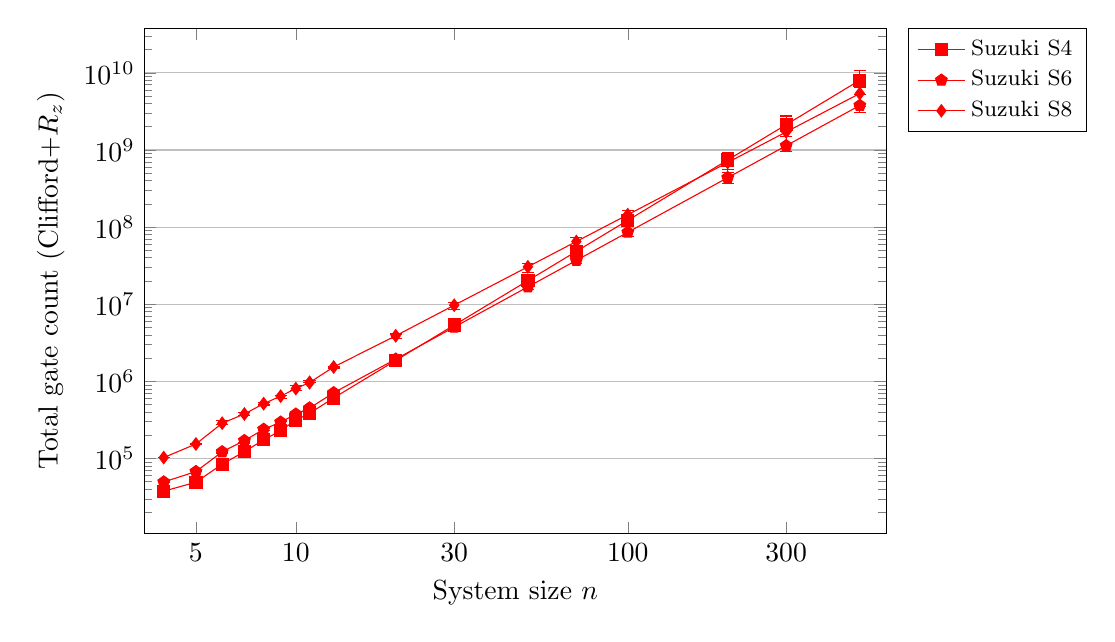
\begin{tikzpicture}
  \begin{loglogaxis}[
    width=11cm, height=8cm,
    xlabel={System size $n$},
    ylabel={Total gate count (Clifford+$R_z$)},
    xtick={5,10,30,100,300}, xticklabels={5,10,30,100,300},
    xmin=3.5, xmax=600,
    ymajorgrids=true,
    legend pos=outer north east,
    legend cell align=left,
    legend style={font=\footnotesize},
  ]
    % suzuki4: measured n, mean over seeds, bars min..max over seeds
    \addplot[red, solid, mark=square*, mark size=2.2pt, mark options={solid, fill=red}, error bars/.cd, y dir=both, y explicit, error bar style={solid}] coordinates {
      (4,37651.2) += (0,508.8) -= (0,339.2)
      (5,49184) += (0,1696) -= (0,1484)
      (6,84333.6) += (0,5978.4) -= (0,4197.6)
      (7,122578) += (0,9497.6) -= (0,8310.4)
      (8,174349) += (0,7123.2) -= (0,6444.8)
      (9,229914) += (0,10494) -= (0,12402)
      (10,315032) += (0,24168) -= (0,11872)
      (11,384780) += (0,16324) -= (0,9328)
    };
    \addlegendentry{Suzuki S4}
    % suzuki4: extrapolated, r = ceil(3.65267 n^1.59931), per step = 212 n + 0; bars min..max of per-seed fits
    \addplot[red, solid, mark=square*, mark size=2.2pt, mark options={solid, fill=red}, forget plot, error bars/.cd, y dir=both, y explicit, error bar style={solid}] coordinates {
      (11,384780)
      (13,609076) += (0,27560) -= (0,19292)
      (20,1.8656e+06) += (0,139920) -= (0,101760)
      (30,5.35512e+06) += (0,553320) -= (0,407040)
      (50,2.0193e+07) += (0,2.9044e+06) -= (0,2.0352e+06)
      (70,4.84229e+07) += (0,8.26588e+06) -= (0,5.66888e+06)
      (100,1.22345e+08) += (0,2.45072e+07) -= (0,1.63664e+07)
      (200,7.41406e+08) += (0,1.92369e+08) -= (0,1.22706e+08)
      (300,2.12697e+09) += (0,6.28432e+08) -= (0,3.9025e+08)
      (500,8.02431e+09) += (0,2.74604e+09) -= (0,1.65e+09)
    };
    % suzuki6: measured n, mean over seeds, bars min..max over seeds
    \addplot[red, solid, mark=pentagon*, mark size=2.2pt, mark options={solid, fill=red}, error bars/.cd, y dir=both, y explicit, error bar style={solid}] coordinates {
      (4,49536) += (0,0) -= (0,0)
      (5,67596) += (0,4644) -= (0,516)
      (6,121982) += (0,8049.6) -= (0,4334.4)
      (7,170486) += (0,10113.6) -= (0,11558.4)
      (8,238598) += (0,9081.6) -= (0,7430.4)
      (9,295358) += (0,11145.6) -= (0,16718.4)
      (10,375648) += (0,26832) -= (0,14448)
      (11,449539) += (0,15892.8) -= (0,6811.2)
    };
    \addlegendentry{Suzuki S6}
    % suzuki6: extrapolated, r = ceil(1.63295 n^1.35284), per step = 1032 n + 0; bars min..max of per-seed fits
    \addplot[red, solid, mark=pentagon*, mark size=2.2pt, mark options={solid, fill=red}, forget plot, error bars/.cd, y dir=both, y explicit, error bar style={solid}] coordinates {
      (11,449539)
      (13,711048) += (0,40248) -= (0,13416)
      (20,1.94016e+06) += (0,165120) -= (0,61920)
      (30,5.04648e+06) += (0,588240) -= (0,278640)
      (50,1.677e+07) += (0,2.7348e+06) -= (0,1.3932e+06)
      (70,3.69869e+07) += (0,7.15176e+06) -= (0,3.68424e+06)
      (100,8.5656e+07) += (0,1.92984e+07) -= (0,1.00104e+07)
      (200,4.37155e+08) += (0,1.28174e+08) -= (0,6.5016e+07)
      (300,1.13499e+09) += (0,3.78641e+08) -= (0,1.89785e+08)
      (500,3.77506e+09) += (0,1.46028e+09) -= (0,7.15692e+08)
    };
    % suzuki8: measured n, mean over seeds, bars min..max over seeds
    \addplot[red, solid, mark=diamond*, mark size=2.2pt, mark options={solid, fill=red}, error bars/.cd, y dir=both, y explicit, error bar style={solid}] coordinates {
      (4,102640) += (0,0) -= (0,0)
      (5,153960) += (0,0) -= (0,0)
      (6,286366) += (0,21554.4) -= (0,9237.6)
      (7,377202) += (0,17962) -= (0,17962)
      (8,513200) += (0,20528) -= (0,20528)
      (9,642013) += (0,4618.8) -= (0,41569.2)
      (10,805724) += (0,66716) -= (0,35924)
      (11,965329) += (0,50806.8) -= (0,5645.2)
    };
    \addlegendentry{Suzuki S8}
    % suzuki8: extrapolated, r = ceil(0.896539 n^1.24879), per step = 5132 n + 0; bars min..max of per-seed fits
    \addplot[red, solid, mark=diamond*, mark size=2.2pt, mark options={solid, fill=red}, forget plot, error bars/.cd, y dir=both, y explicit, error bar style={solid}] coordinates {
      (11,965329)
      (13,1.53447e+06) += (0,0) -= (0,66716)
      (20,3.90032e+06) += (0,205280) -= (0,307920)
      (30,9.69948e+06) += (0,769800) -= (0,1.07772e+06)
      (50,3.05354e+07) += (0,3.0792e+06) -= (0,4.8754e+06)
      (70,6.50224e+07) += (0,7.54404e+06) -= (0,1.18549e+07)
      (100,1.44722e+08) += (0,1.95016e+07) -= (0,3.02788e+07)
      (200,6.87688e+08) += (0,1.15983e+08) -= (0,1.7962e+08)
      (300,1.71204e+09) += (0,3.24856e+08) -= (0,4.97291e+08)
      (500,5.39886e+09) += (0,1.17523e+09) -= (0,1.75001e+09)
    };
  \end{loglogaxis}
\end{tikzpicture}
